%%% ====================== %%%
%%%      INTRODUCTION      %%%
%%% ====================== %%%

% FIGURE 0-01 - LENGTH SCALES IN ATMOSPHERIC SCIENCES

\begin{figure}
\centering
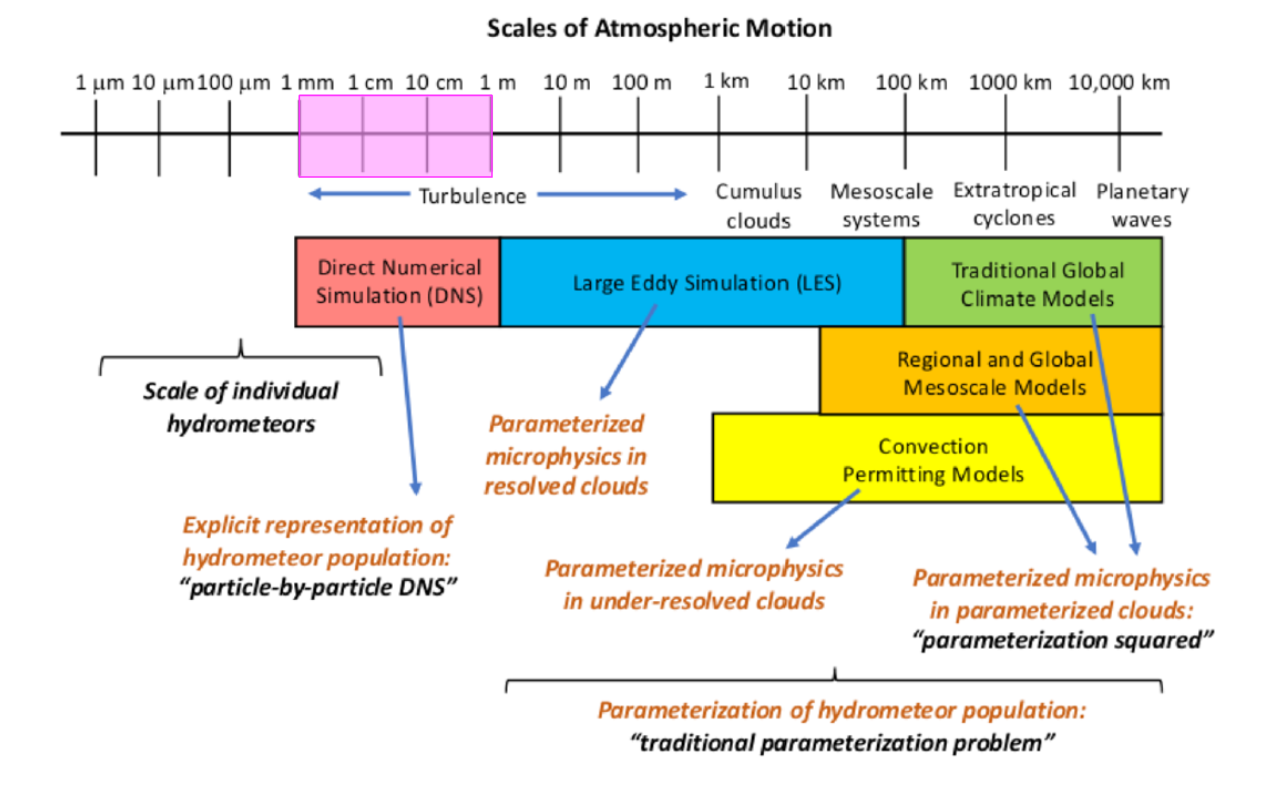
\includegraphics[width=13cm]{figures/0-01_atmo-scales.png}
\caption{
Hierarchy of atmospheric models and the scales of atmospheric motion reproduced from \textcite{Morrison2020} with author's permission.
Coloured rectangles represent types of simulations commonly used when working with respective length scales, and comments emphasise transition from directly resolving most elements of the model (left) to including more and more parameterisations with the increase of scale (right).
Magenta rectangle positioned on the axis was added to emphasise range of scales that corresponds to simulations discussed in this thesis.}
\label{fig:atmo-scales}
\end{figure}



%%% =================== %%%
%%%      CHAPTER 1      %%%
%%% =================== %%%

% FIGURE 1-01 - DETERMINISTIC FORCING ENERGY SPECTRUM

\begin{figure}
\centering
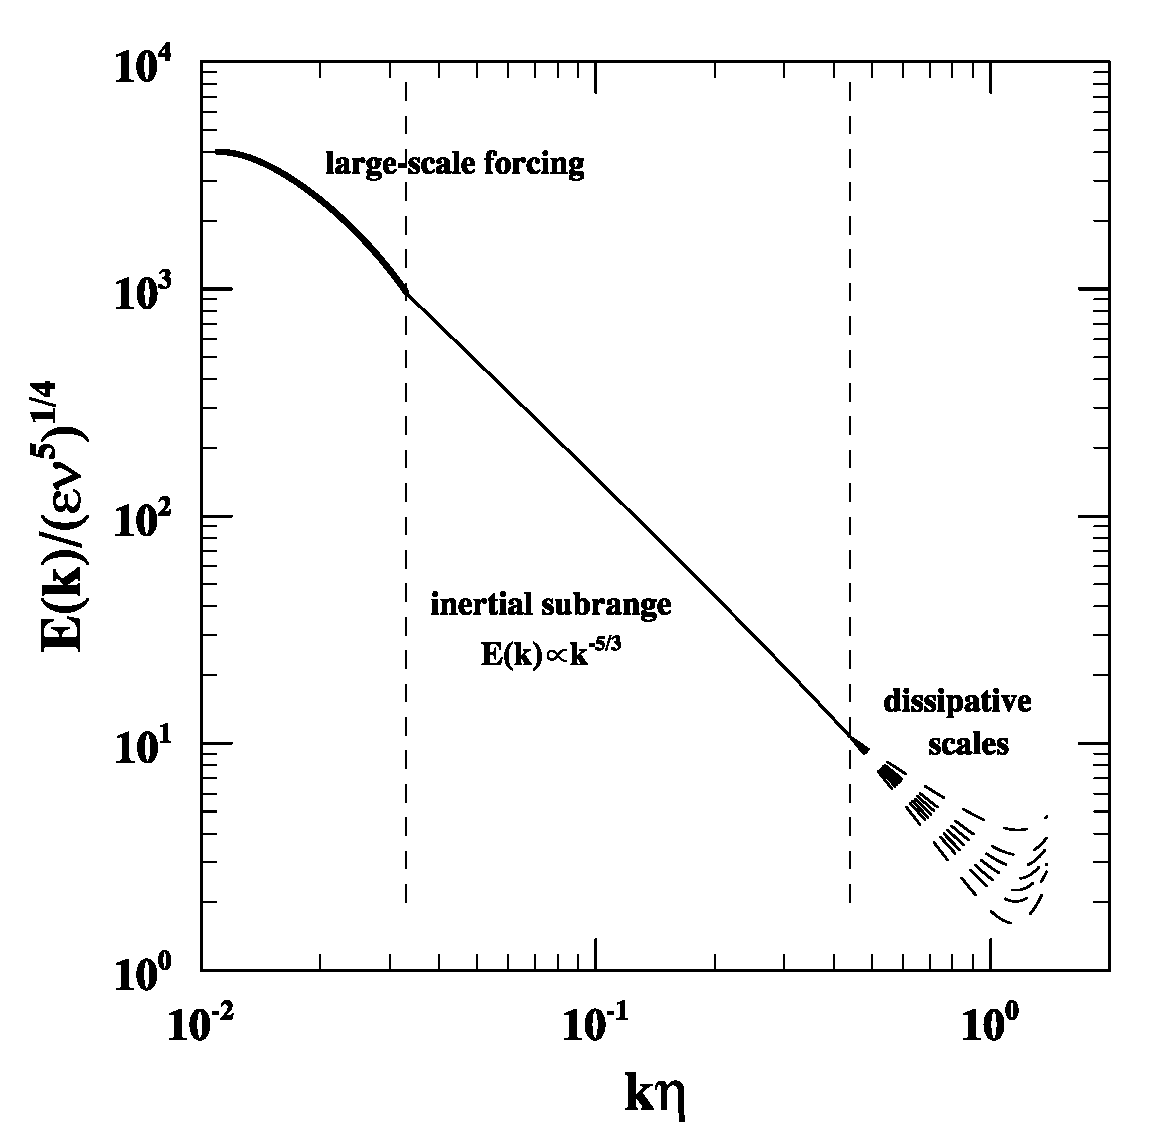
\includegraphics[width=10cm]{figures/1-01_forcing.pdf}
\caption{
The basic idea of deterministic forcing scheme: energy is supplied on large scales by fixing it for small wavenumbers (bold line), then it is transferred following Kolmogorov energy cascade ($E(k) \propto k^{-5/3}$) in inertial subrange, to finally reach smallest dissipative eddies represented by largest resolved wavenumbers (when $k_{\max} \eta \sim 1 = 10^0$, diverging dashed lines) that have largest influence on measured particle statistics at contact distances.
Both axes are using standard normalisations (see Section \ref{ssc:ch2.flow.spec}) and logarithmic scale, that makes $k^{-5/3}$ curves appear as straight lines.}
\label{fig:forcing}
\end{figure}

% FIGURE 1-02 - GRID SIZES IN DNS VS LES

\begin{figure}
\centering
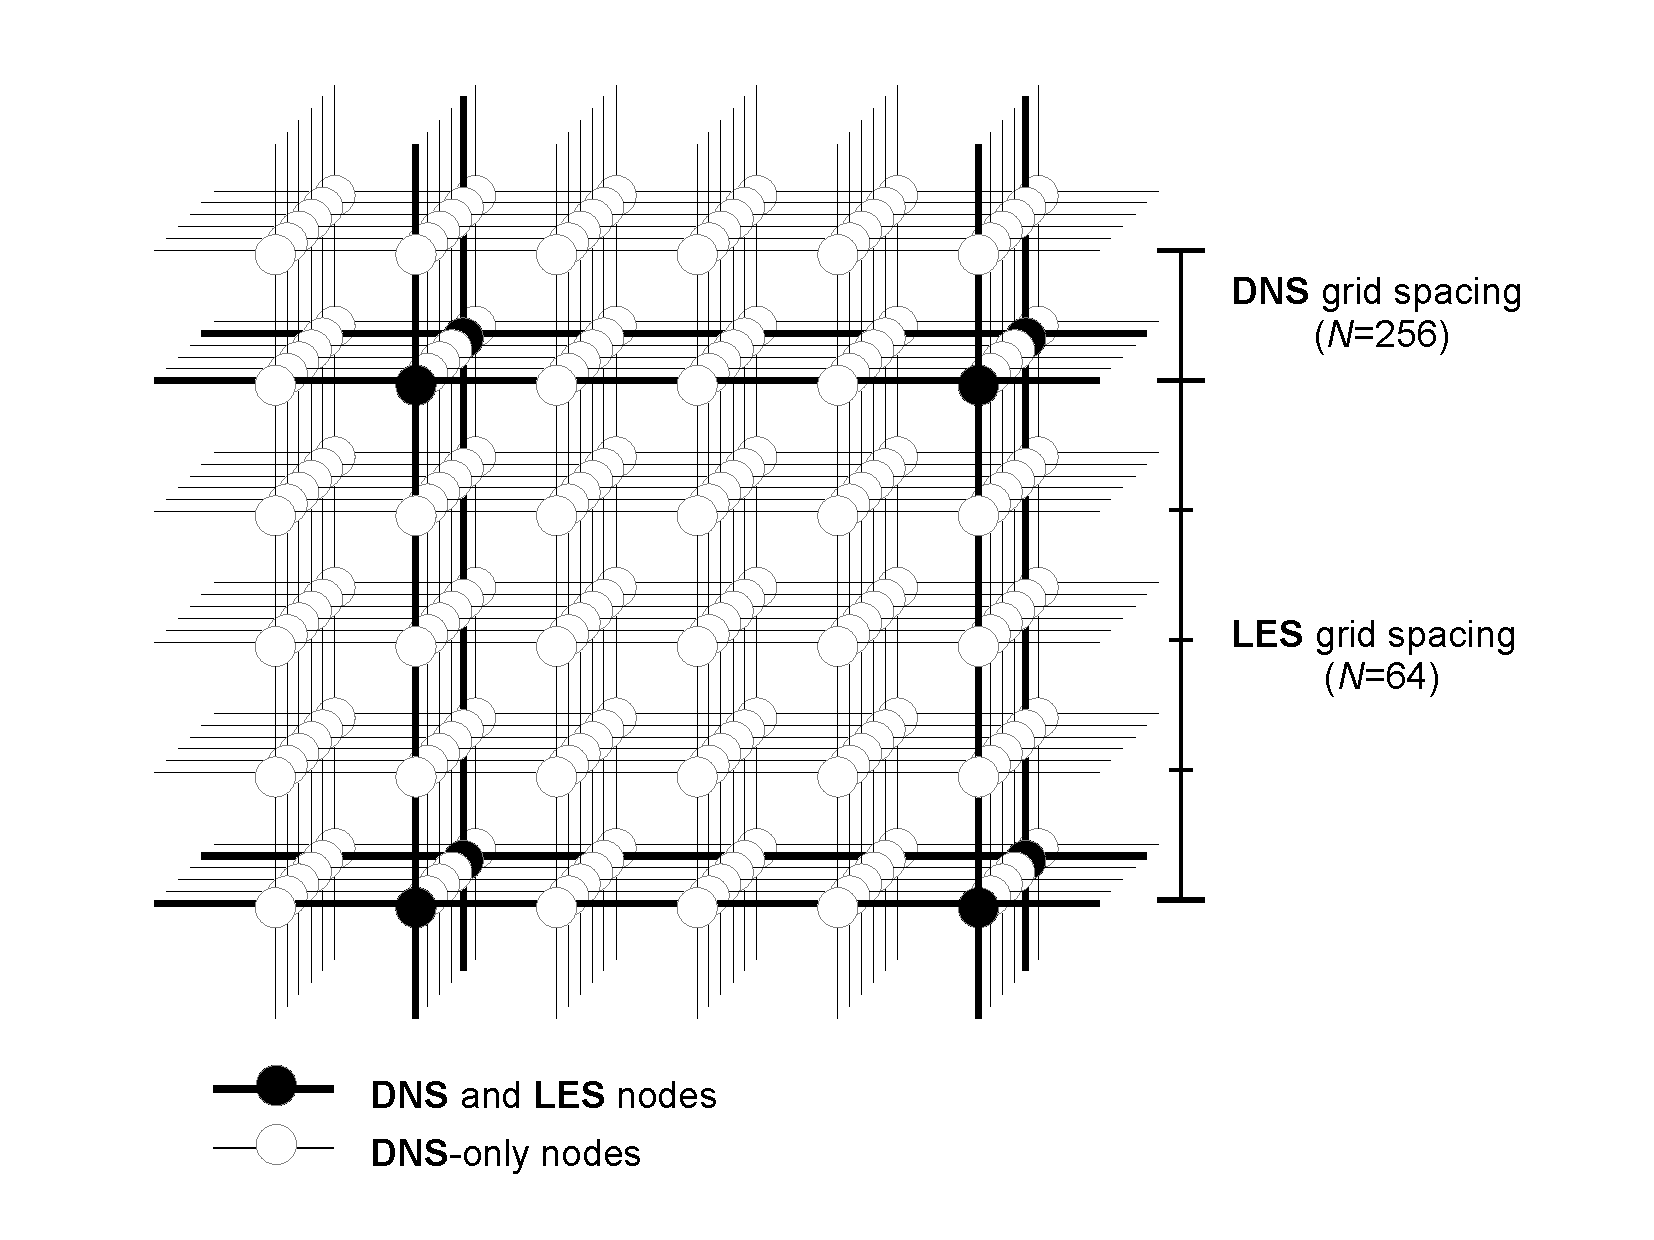
\includegraphics[width=17cm]{figures/1-02_dns-les-grids.pdf}
\caption{
Conceptual juxtaposition of computational grids for DNS and LES.
In LES, the subgrid-scale modelling parameterises small-scale turbulence that is directly resolved by $4 \times 4 \times 4$ block of cells in DNS.
}
\label{fig:dns-les-grids}
\end{figure}

% FIGURE 1-03 - PROJECTION ONTO NEIGHBOURING NODES

\begin{figure}[h]
\centering
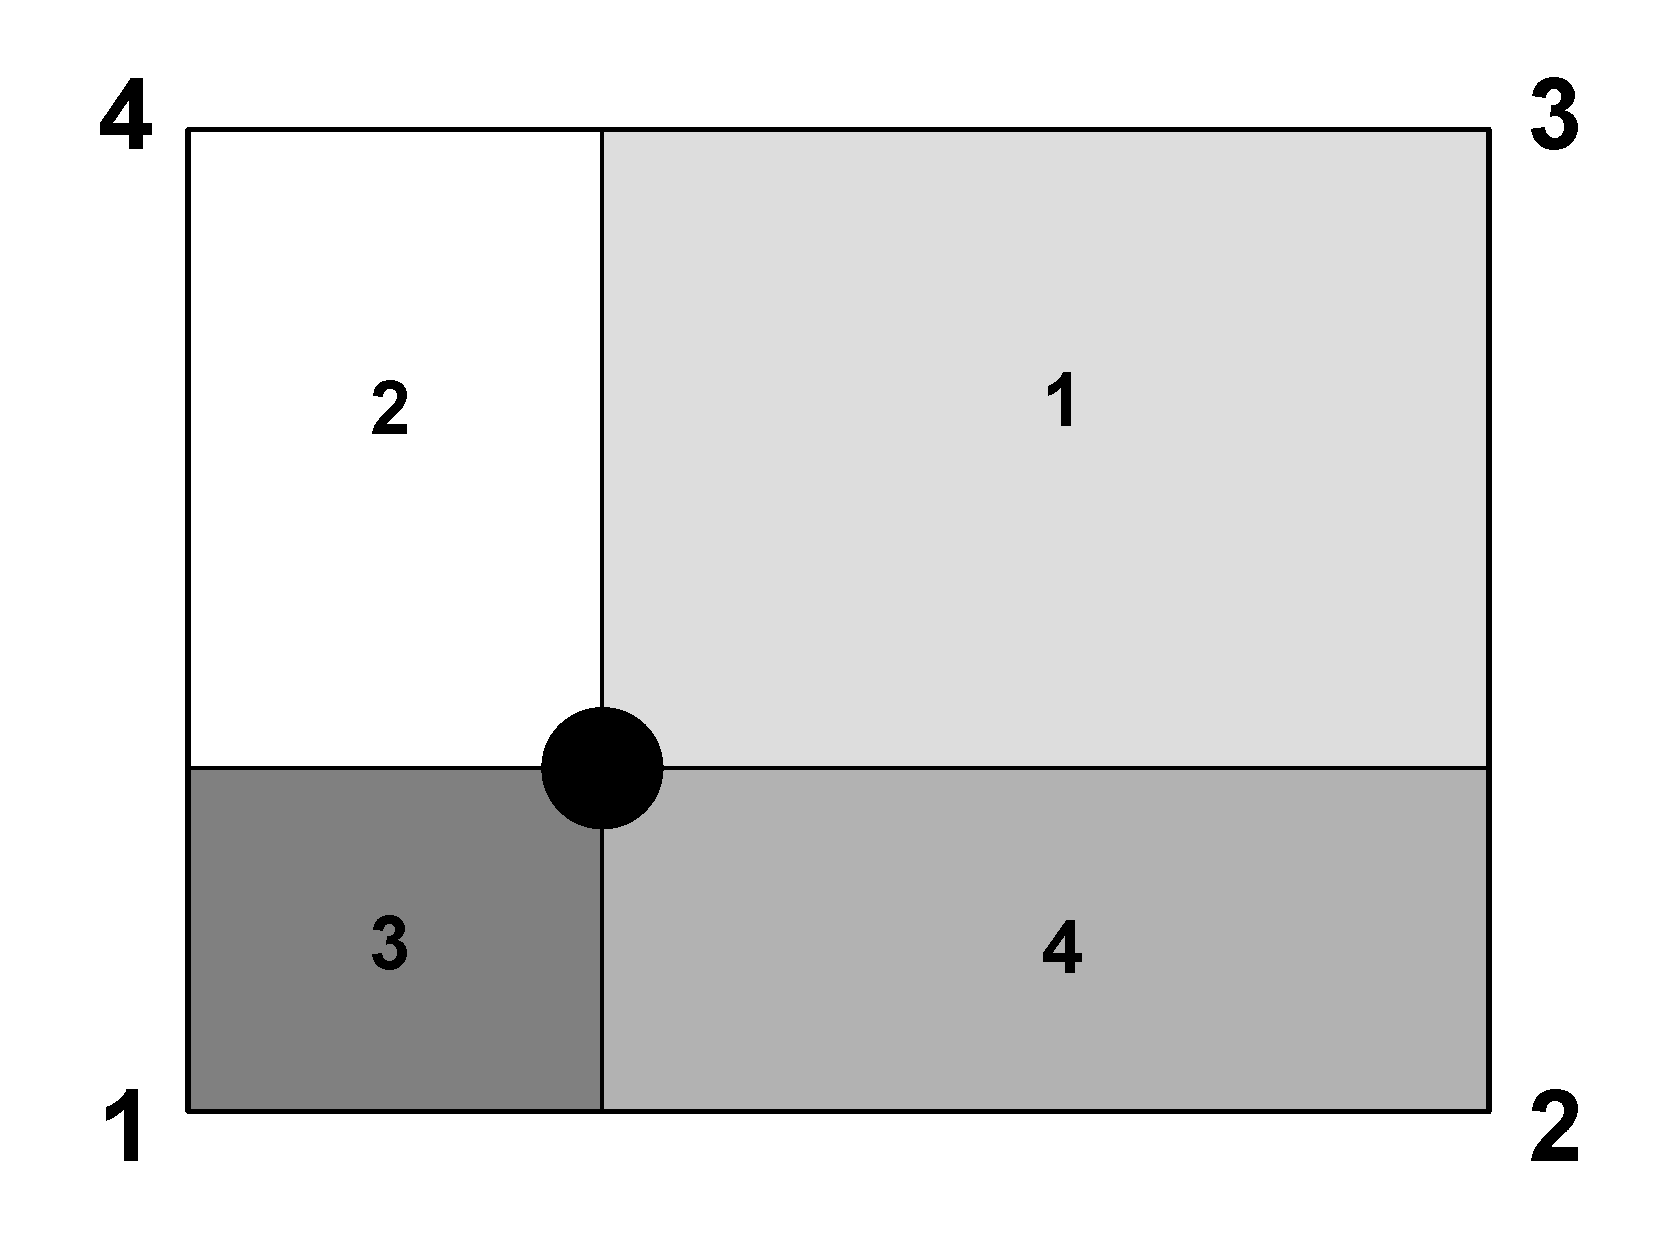
\includegraphics[width=8cm]{figures/1-03_pnn.pdf}
\caption{
Projection onto neighbouring nodes (PNN; simplified illustration for 2D case).
The contribution of the particle momentum to the fluid momentum at a grid node depends on the separation distance.
For example, the particle force may be projected onto neighbouring nodes using weights that are proportional to cell areas (or volumes in 3D case).
Here, the fluid flow at grid node $1$ is affected by a fraction of the particle Stokes drag proportional to the area with marker $1$, and so on.
Based on \textcite[Fig. 1 therein]{Garg2007}.}
\label{fig:pnn}
\end{figure}

% FIGURE 1-04 - 2D DOMAIN DECOMPOSITION

\begin{figure}[h]
\centering
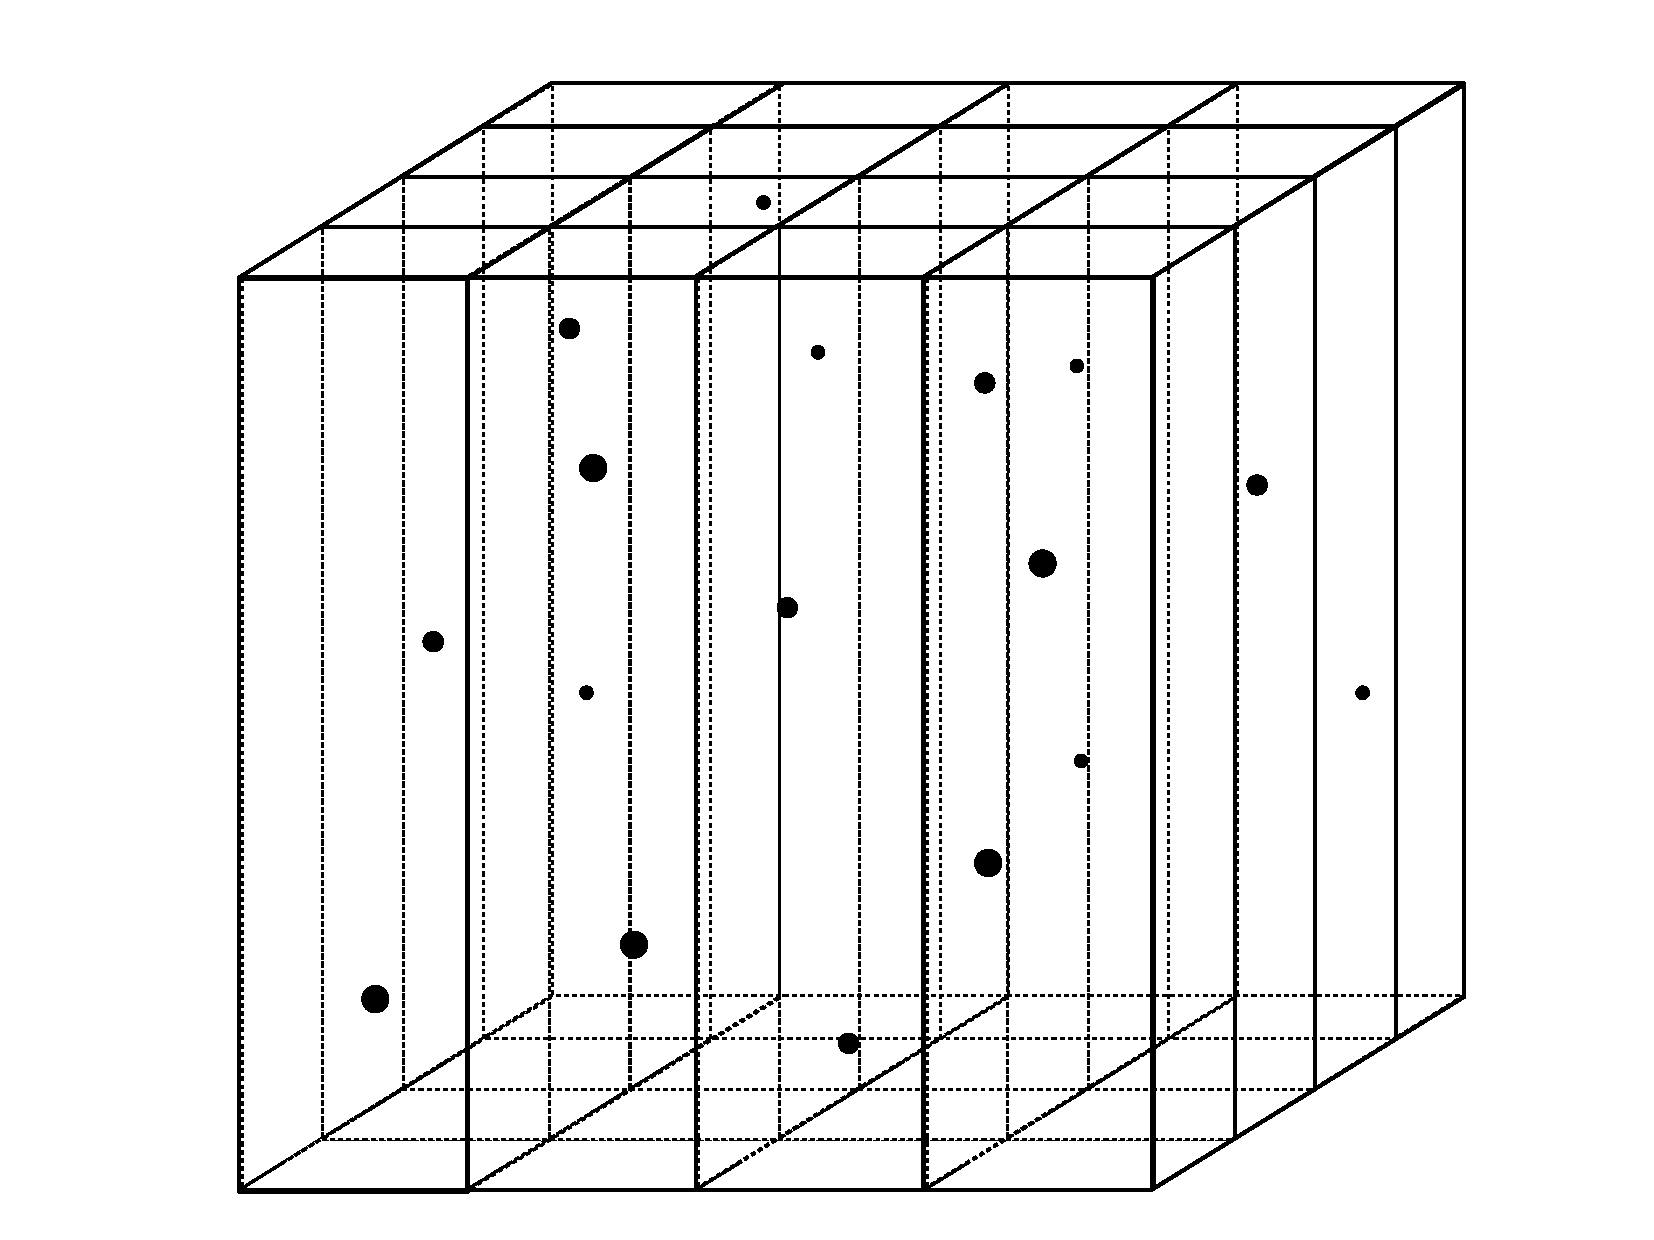
\includegraphics[width=10cm]{figures/1-04_2dd.pdf}
\caption{
Schematic representation of 2D domain decomposition.
This image corresponds to the actual decomposition of $64^{3}$ grid used for LES.
Entire domain is divided into $4 \times 4 = 16$ subdomains, each~with~$16 \times 16 \times 64$ nodes.
}
\label{fig:2dd}
\end{figure}